\documentclass{weekly}
\begin{document}
\maketitlew{Аналитическая механика}{1}{6}{23}

\begin{wrapfigure}{r}{.28\textwidth}
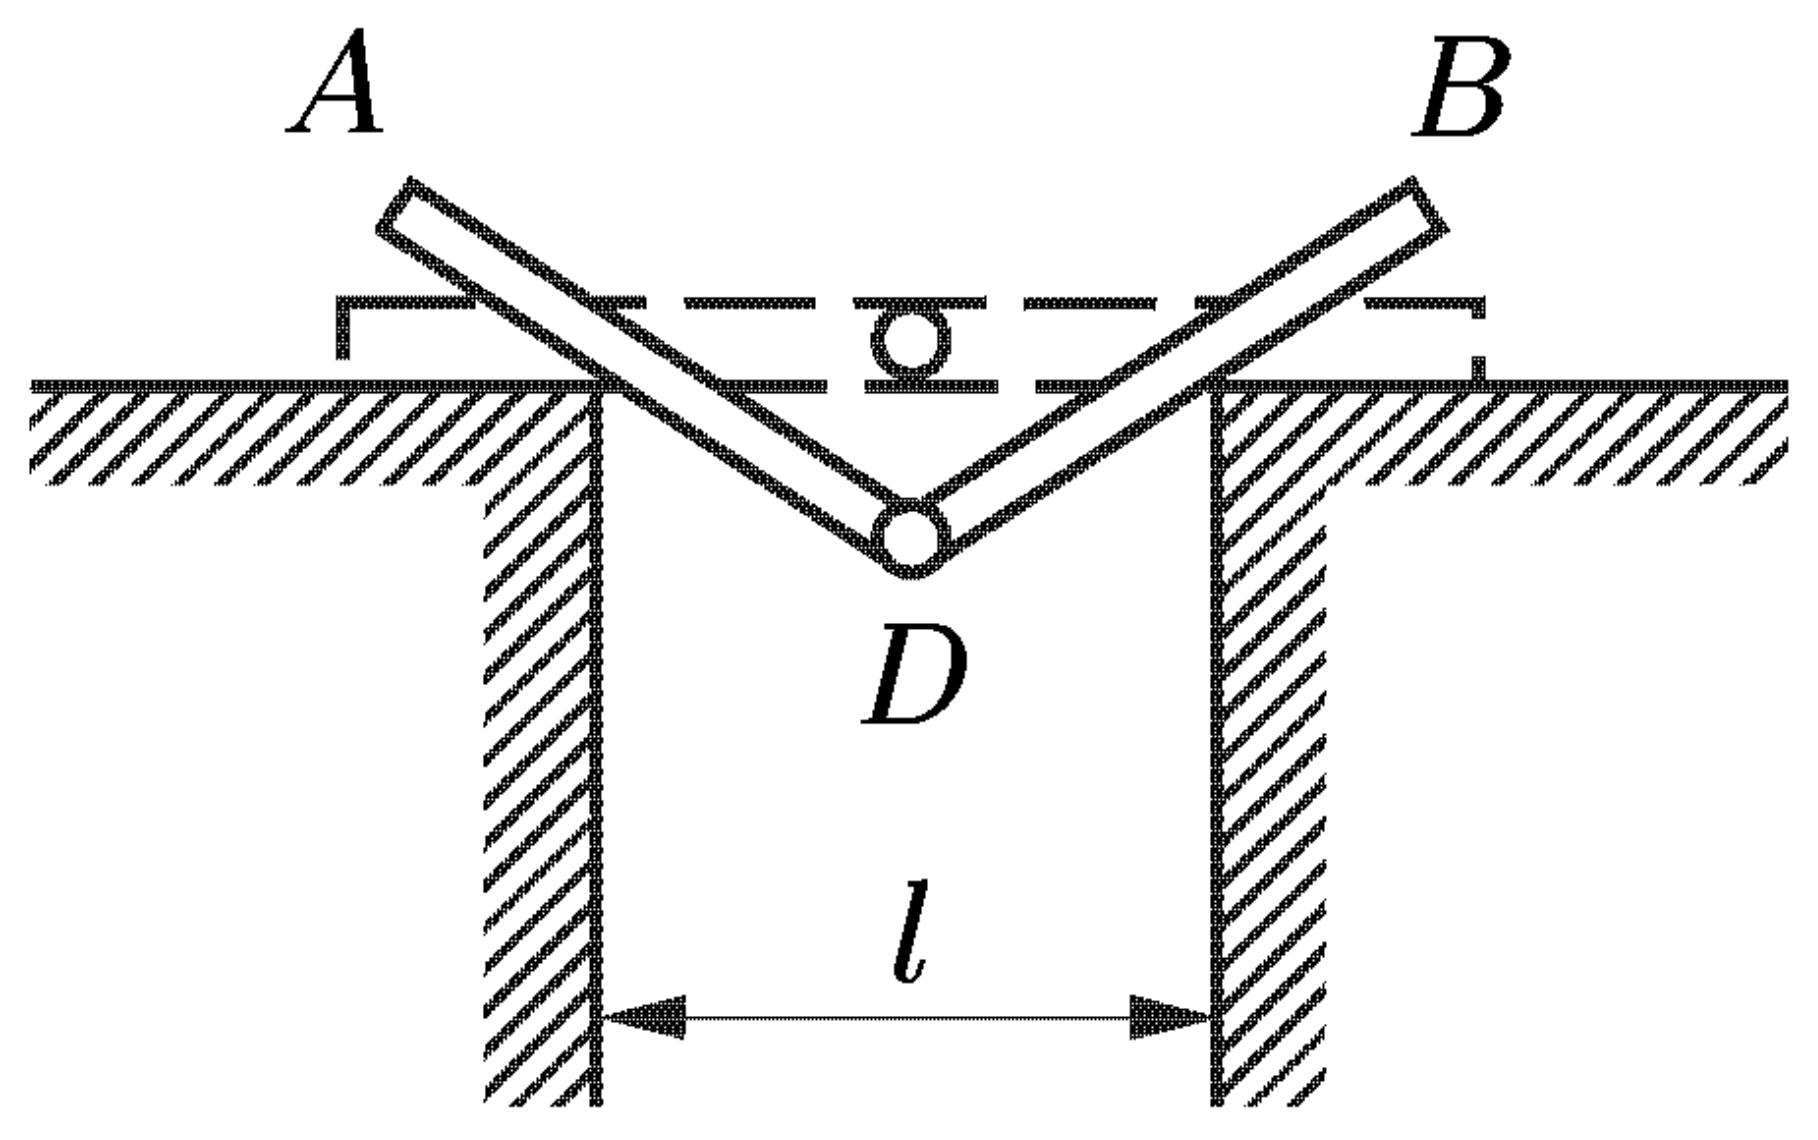
\includegraphics[width=\linewidth]{7-29}
\end{wrapfigure}
\paragraph{7.29.} Однородные стержни~$AD$ и~$BD$, шарнирно соединённые
в~точке~$D$, опираются на~два гладких угла. Длина каждого стержня
равна расстоянию между опорами~$l$. В~начальный момент стержни
горизонтальны и~расположены симметрично относительно опор,
а~затем (после малого начального толчка) приходят в~движение
за~счёт собственного веса, причём точка~$D$ перемещается по~вертикали.
Определить скорость точки~$D$ в~момент, когда концы стержней~$A$ и~$B$
достигнут угловых точек.

$\blacktriangleright$ При~решении задачи~3.12 было показано,
что~скорость~$v_T$ точки касания стержня вершины угла
направлена вдоль стержня и~связана со~скоростью точки~$D$
и~углом между стержнями~$\varphi$ соотношением
\begin{equation}
    v_T = v_D \cos\frac\varphi 2.
\end{equation}

Применив закон сохранения энергии и~теорему Кёнига, получим
для~рассматриваемого момента времени ($\varphi\to\varphi_0 = 60^\circ$):
\begin{equation}
    0 = -2 \cdot g\frac{l \cos\frac{\varphi_0}{2}}{2} +
            2 \cdot \frac{v_C^2}{2} +
            2 \cdot \frac{l^2}{12} \frac{\omega^2}{2}.
    \label{7.29:energy}
\end{equation}

$\triangleright$ Пусть концы~$\vec r_1$ и~$\vec r_2$ однородного стержня,
совершающего плоскопараллельное движение, имеют скорости~$\vec v_1$
и~$\vec v_2$. Найдём скорость~$\vec v_C$ его центра масс
и~угловую скорость~$\omega$:
\begin{align}
    \vec r_C = \dfrac{\vec r_1 + \vec r_2}{2}
&\then
    \vec v_C = \dfrac{\vec v_1 + \vec v_2}{2};
\\
    \vec v_2 - \vec v_1 = \vec\omega \times (\vec r_2 - \vec r_1)
&\then
    \vec\omega \times (\vec v_2 - \vec v_1)
        = -\omega^2 (\vec r_2 - \vec r_1).
\end{align}
Последнее соотношение скаляризируем как
\begin{equation}
    \omega = \frac{\abs{v_2^{\perp} - v_1^{\perp}}}{l},
\end{equation}
что, в~общем-то, и~так было понятно. \hfill $\triangleleft$

Выполним соответствующие подстановки в~\eqref{7.29:energy}:
\begin{gather}
    \frac{\sqrt{3}}{2} gl = v_C^2 + \frac{1}{3} \omega^2 l^2
        = \left(v_T^2 + \frac{1}{4} \omega^2 l^2\right)
            + \frac{1}{12} \omega^2 l^2
        = v_D^2 \left(\cos^2\frac{\varphi_0}{2}
            + \frac{1}{3} \sin^2\frac{\varphi_0}{2}\right).
\end{gather}
\textbf{Ответ:}\qquad $v_D = \sqrt{\dfrac{3\sqrt{3}}{5}}$.
\hfill $\blacktriangleleft$

\end{document}
